\documentclass[dvipdfmx,cjk,10.2pt]{beamer} 
%\documentclass[dvipdfm,cjk]{beamer} %% オプションは環境や利用するプログラムに
%\documentclass[dvips,cjk]{beamer}   %% よって変える

\usepackage{tikz}
\usepackage{subfigure}
\usepackage[all]{xy}
\usepackage{wrapfig}

\newcommand{\R}{\mathbb{R}}
\newcommand{\Q}{\mathbb{Q}}
\newcommand{\Z}{\mathbb{Z}}
\newcommand{\N}{\mathbb{N}}



\makeatletter
\newcommand\xleftrightarrow[2][]{%
  \ext@arrow 9999{\longleftrightarrowfill@}{#1}{#2}}
\newcommand\longleftrightarrowfill@{%
  \arrowfill@\leftarrow\relbar\rightarrow}
\makeatother

\AtBeginDvi{\special{pdf:tounicode 90ms-RKSJ-UCS2}} %% しおりが文字化けしないように
%\AtBeginDvi{\special{pdf:tounicode EUC-UCS2}}

\setbeamertemplate{navigation symbols}{} %% 右下のアイコンを消す
\setbeamertemplate{theorems}[normal font] %%斜体を直す

\usetheme{CambridgeUS}         %% theme の選択
%\usetheme{Boadilla}           %% Beamer のディレクトリの中の
%\usetheme{Madrid}             %% beamerthemeCambridgeUS.sty を指定
%\usetheme{Antibes}            %% 色々と試してみるといいだろう
%\usetheme{Montpellier}        %% サンプルが beamer\doc に色々とある。
%\usetheme{Berkeley}
%\usetheme{Goettingen}
%\usetheme{Singapore}
%\usetheme{Szeged}

%\usecolortheme{rose}          %% colortheme を選ぶと色使いが変わる
%\usecolortheme{albatross}

%\useoutertheme{shadow}                 %% 箱に影をつける
\usefonttheme{professionalfonts}       %% 数式の文字を通常の LaTeX と同じにする

%\setbeamercovered{transparent}         %% 消えている文字をうっすらと表示する


\theoremstyle{definition}
\setbeamertemplate{theorems}[numbered]  %% 定理に番号をつける
\newtheorem{Thm}{定理}[section]
%\theoremstyle{example}
\newtheorem{Ex}[Thm]{例}
%\newtheorem{exam}[thm]{Example}
\newtheorem{Rem}[Thm]{注意}
\newtheorem{Conj}[Thm]{予想}
\newtheorem{Def}[Thm]{定義}
\newtheorem{Prob}[Thm]{問題}

\setbeamercolor{block title}{fg=blue!70!black, bg=blue!15!white} 
\setbeamercolor{block body}{fg=black, bg=blue!10!white}



\begin{document}
\title{微分・積分 第13回} 
\author{慶応義塾大学}            %% ここに書かれた情報は色々なところに使われるので
\institute[]{総合政策学部・環境情報学部}   %% なるべく設定した方が良い
\date{}



\begin{frame}                  %% \begin{frame}..\end{frame} で 1 枚のスライド
\titlepage                     %% タイトルページ
\end{frame}

%\begin{frame}                  %% 目次 (必要なければ省略)
%\tableofcontents
%\end{frame}






%%%%%%%%%%%%%%%%%%%%%%%%%%%%%%%%%%%%%%%%%%%%%%%%%%%%%%%%%%%%%%%%%%%%%%%%%%%%%%%%%%%%%%%
%%%%%%%%%%%%%%%%%%%%%%%%%%%%%%%%%%%%%%%%%%%%%%%%%%%%%%%%%%%%%%%%%%%%%%%%%%%%%%%%%%%%%%%

\section{講義概要}


\begin{frame}
\frametitle{今日の内容}



\begin{enumerate}
\item 有界閉領域, 二重積分, 累次積分
\item 変数変換, ヤコビアン
\end{enumerate} 



\end{frame}




%%%%%%%%%%%%%%%%%%%%%%%%%%%%%%%%%%%%%%%%%%%%%%%%%%%%%%%%%%%%%%%%%%%%%%%%%%%%%%%%%%%%%%%
%%%%%%%%%%%%%%%%%%%%%%%%%%%%%%%%%%%%%%%%%%%%%%%%%%%%%%%%%%%%%%%%%%%%%%%%%%%%%%%%%%%%%%%


%%%%%%%%%%%%%%%%%%%%%%%%%%%%%%%%%%%%%%%%%%%%%%%%%%%%%%%%%%%%%%%%%%%%%%%%%%%%%%%%%%%%%%%
%%%%%%%%%%%%%%%%%%%%%%%%%%%%%%%%%%%%%%%%%%%%%%%%%%%%%%%%%%%%%%%%%%%%%%%%%%%%%%%%%%%%%%%



\section{二変数関数の積分}


\begin{frame}
\frametitle{二変数関数の積分}


集合$D \subset \R^2$とその上で定義された二変数関数$f(x,y)$を考える. 
一変数関数の場合と同様に, $f(x,y)$のグラフと$D$の境界上の点を通り$xy$平面と垂直に交わる直線, および$xy$平面で囲まれた3次元図形の体積
$$
\iint_Df(x,y)dxdy
$$
を定義したい.  

\vspace{-5mm}
\begin{figure}[htbp]
 \begin{center} 
  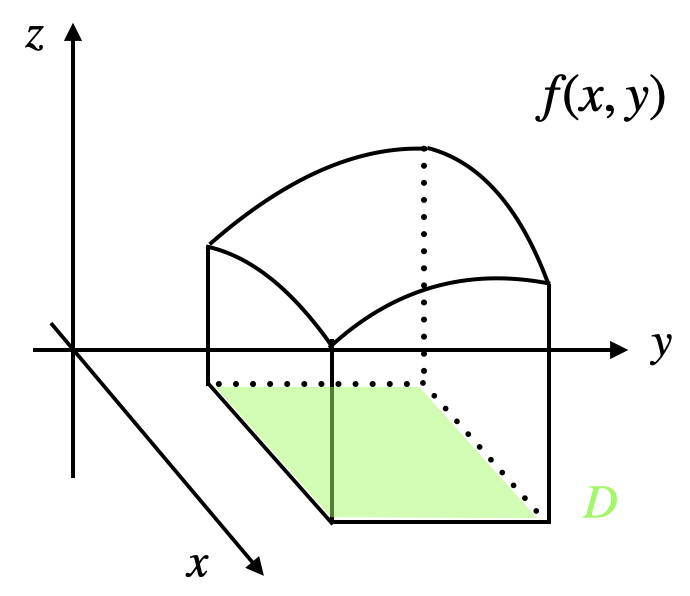
\includegraphics[width=40mm]{volume.png}
 \end{center}
\end{figure}


\end{frame}


%%%%%%%%%%%%%%%%%%%%%%%%%%%%%%%%%%%%%%%%%%%%%%%%%%%%%%%%%%%%%%%%%%%%%%%%%%%%%%%%%%%%%%%
%%%%%%%%%%%%%%%%%%%%%%%%%%%%%%%%%%%%%%%%%%%%%%%%%%%%%%%%%%%%%%%%%%%%%%%%%%%%%%%%%%%%%%%




\begin{frame}
\frametitle{二変数関数の積分}


\begin{Def}
平面内の集合$D \subset R^2$がある正方形$[a,a+l]\times [b,b+l]$に含まれるとき, $D$は\underline{有界}であるという. 
\end{Def}

以下では$D\subset \R^2$を有界な閉領域とする. 
閉領域の厳密な定義は行わないが, 広がりを持ち, 境界を含むような集合である. 
例えば, 線分$[a,b] \times \{0\}$や開円板$\{x^2+y^2<1\}$は閉領域ではない. 
また$D$は面積確定であるとする. 
\vspace{-5mm}

\begin{figure}[htbp]
 \begin{center} 
  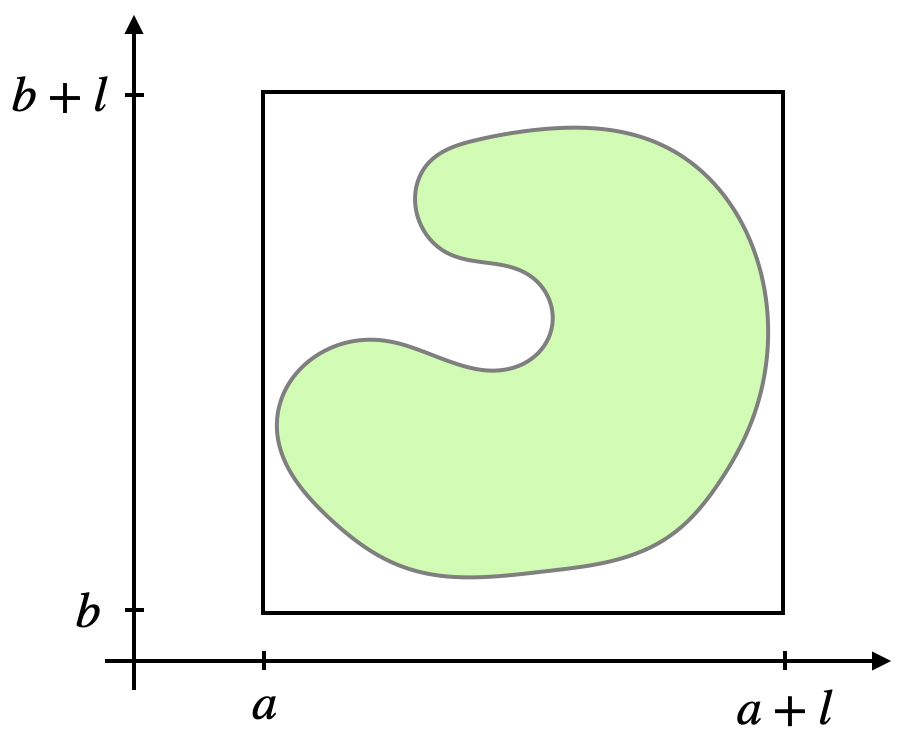
\includegraphics[width=47mm]{bdd_domain.png}
 \end{center}
\end{figure}

\end{frame}



%%%%%%%%%%%%%%%%%%%%%%%%%%%%%%%%%%%%%%%%%%%%%%%%%%%%%%%%%%%%%%%%%%%%%%%%%%%%%%%%%%%%%%%
%%%%%%%%%%%%%%%%%%%%%%%%%%%%%%%%%%%%%%%%%%%%%%%%%%%%%%%%%%%%%%%%%%%%%%%%%%%%%%%%%%%%%%


\begin{frame}
\frametitle{リーマン和}

%定積分の定義は一変数の場合と同様である. 
\vspace{-2mm}
$D$が正方形$[a,a+l]\times [b,b+l]$に含まれるとする. 
正方形の一辺を$n$等分して得られる面積$\Delta s=(l/n)^2$の$n^2$個の正方形$\{s_{ij}\}_{i,j=1}^n$を考える. 

\vspace{-4mm}
\begin{figure}[htbp]
 \begin{center} 
  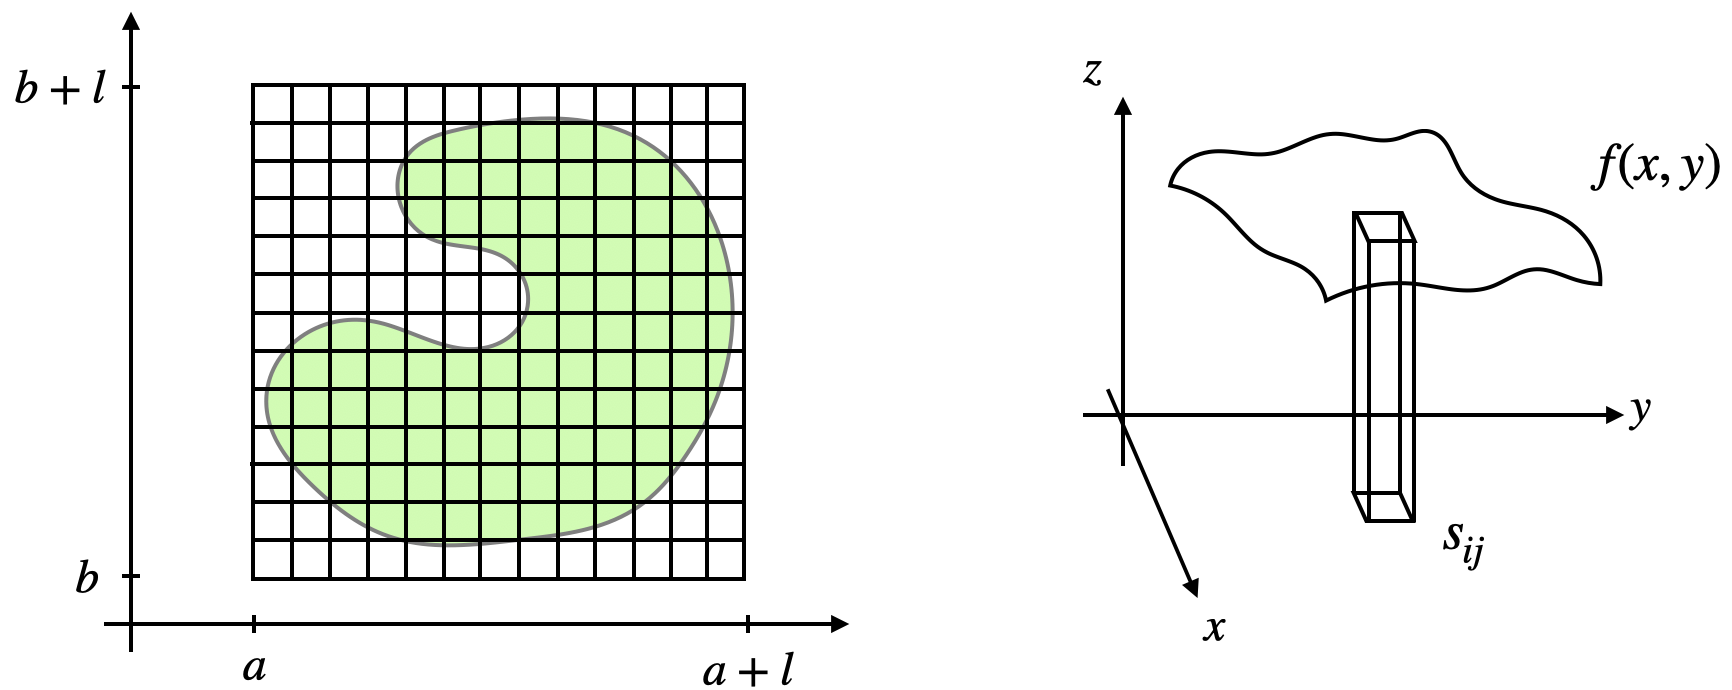
\includegraphics[width=90mm]{div_domain2.png}
 \end{center}
\end{figure}
\vspace{-3mm}

$s_{ij} \cap D \ne \emptyset$であるとき, $(x_{ij},y_{ij})\in s_{ij} \cap D$を取り, $s_{ij}$を底面とする高さ$f(x_{ij},y_{ij})$の直方体の体積の総和 \vspace{-1mm}
$$
\sum_{i,j }f(x_{ij},y_{ij})\Delta s \vspace{-4mm}
$$
を\underline{リーマン和}と呼ぶ. 

\end{frame}




%%%%%%%%%%%%%%%%%%%%%%%%%%%%%%%%%%%%%%%%%%%%%%%%%%%%%%%%%%%%%%%%%%%%%%%%%%%%%%%%%%%%%%%
%%%%%%%%%%%%%%%%%%%%%%%%%%%%%%%%%%%%%%%%%%%%%%%%%%%%%%%%%%%%%%%%%%%%%%%%%%%%%%%%%%%%%%


\begin{frame}
\frametitle{二重積分}


\begin{Def}
$n \to \infty$のとき, リーマン和$\sum_{i,j }f(x_{ij},y_{ij})\Delta s$が$(x_{ij},y_{ij})$の取り方に依らずある値に収束するとき, 
$f(x)$は領域$D$で\underline{二重積分可能}であるといい, その極限値を
$$
\iint_D f(x,y)dxdy
$$
と表す. この値を$f(x)$の\underline{二重積分}という. 
\end{Def}

\begin{itemize}
\item 一変数関数の場合と同様に, 二重積分は$xy$平面の上の部分の体積を正, 下の部分の体積を負として足し合わせた符号付き体積を表す. 
\item 特に$f(x ,y)=1$のとき, 二重積分の値は$D$の面積と一致する. 
\end{itemize}

\end{frame}



%%%%%%%%%%%%%%%%%%%%%%%%%%%%%%%%%%%%%%%%%%%%%%%%%%%%%%%%%%%%%%%%%%%%%%%%%%%%%%%%%%%%%%%
%%%%%%%%%%%%%%%%%%%%%%%%%%%%%%%%%%%%%%%%%%%%%%%%%%%%%%%%%%%%%%%%%%%%%%%%%%%%%%%%%%%%%%


\begin{frame}
\frametitle{二重積分}

二重積分は一変数の場合と同じく, 極限によって定義されているため, 
定義から積分可能性を確認することは難しいが, 次の定理が知られている. 

\begin{Thm}
有界な閉領域$D$で定義された連続関数$f(x,y)$は$D$で二重積分可能である. 
\end{Thm}

以下では, 関数は全て連続であると仮定し, 具体的な計算方法を解説する. 

\end{frame}

%%%%%%%%%%%%%%%%%%%%%%%%%%%%%%%%%%%%%%%%%%%%%%%%%%%%%%%%%%%%%%%%%%%%%%%%%%%%%%%%%%%%%%%
%%%%%%%%%%%%%%%%%%%%%%%%%%%%%%%%%%%%%%%%%%%%%%%%%%%%%%%%%%%%%%%%%%%%%%%%%%%%%%%%%%%%%%%

\section{累次積分}


\begin{frame}
\frametitle{累次積分}


領域$D$の形状によっては二重積分は一変数関数の積分の繰り返しで求めることができる. 
このような積分を\underline{累次積分}と呼ぶ. 
$D$が長方形の場合は次のように計算できる.  


\begin{Thm}
$D=[a,b]\times [c,d]$であれば
\begin{align*}
\iint_Df(x,y)dxdy &= \int_a^b\big( \int_c^d f(x,y)dy\big)dx \\
& = \int_c^d\big( \int_a^b f(x,y)dx\big)dy.
\end{align*}
\end{Thm}

\end{frame}


%%%%%%%%%%%%%%%%%%%%%%%%%%%%%%%%%%%%%%%%%%%%%%%%%%%%%%%%%%%%%%%%%%%%%%%%%%%%%%%%%%%%%%%
%%%%%%%%%%%%%%%%%%%%%%%%%%%%%%%%%%%%%%%%%%%%%%%%%%%%%%%%%%%%%%%%%%%%%%%%%%%%%%%%%%%%%%%



\begin{frame}
\frametitle{累次積分}

例えば, 積分$\int_a^b\big( \int_c^d f(x,y)dy\big)dx$は, $x$を固定した$y$の関数$f(x,y)$のグラフの面積$\int_c^d f(x,y)dy$を計算し, 
それを$x$方向に積分することで体積を計算している. 

\begin{figure}[htbp]
 \begin{center} 
  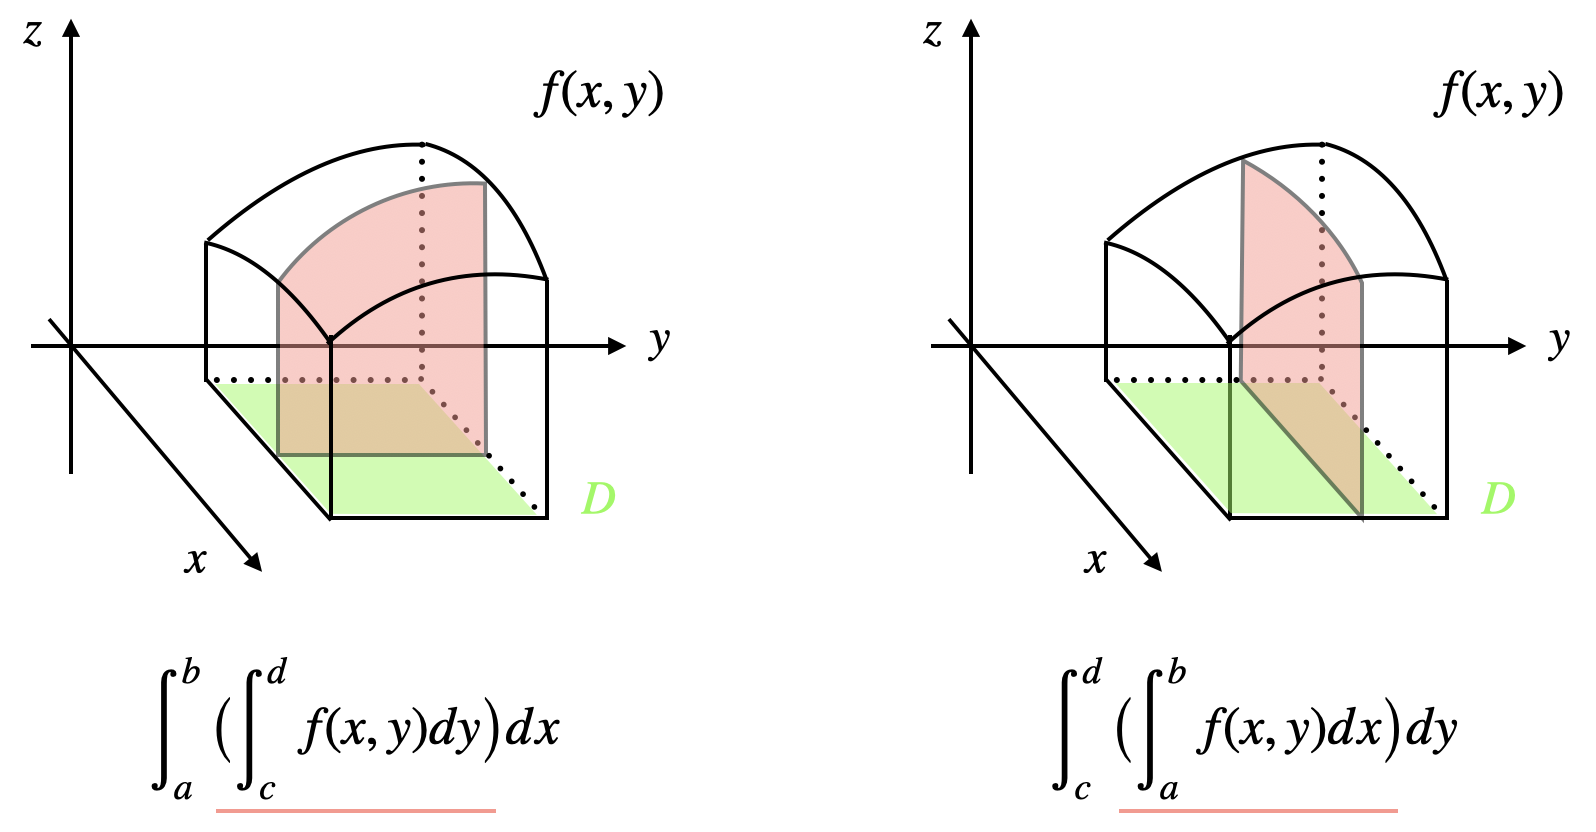
\includegraphics[width=100mm]{2dir.png}
 \end{center}
\end{figure}

\end{frame}

%%%%%%%%%%%%%%%%%%%%%%%%%%%%%%%%%%%%%%%%%%%%%%%%%%%%%%%%%%%%%%%%%%%%%%%%%%%%%%%%%%%%%%%
%%%%%%%%%%%%%%%%%%%%%%%%%%%%%%%%%%%%%%%%%%%%%%%%%%%%%%%%%%%%%%%%%%%%%%%%%%%%%%%%%%%%%%%



\begin{frame}
\frametitle{累次積分}



$D=[0,1]\times [0,2]$であるとき
\begin{align*}
\iint_Dxy^2 dxdy &= \int_0^1\big( \int_0^2 xy^2dy\big)dx = \int_0^1\big[\frac{1}{3}xy^3\big]_{y=0}^2dx\\
& = \int_0^1 \frac{8}{3}xdx  = \big[ \frac{4}{3}x^2\big]_0^1=\frac{4}{3}. 
\end{align*}
\begin{align*}
\iint_Dxy^2 dxdy &= \int_0^2\big( \int_0^1 xy^2dx\big)dy = \int_0^2\big[\frac{1}{2}x^2y^2\big]_{x=0}^1dy\\
& = \int_0^2 \frac{1}{2}y^2dy  = \big[ \frac{1}{6}y^3\big]_0^2=\frac{4}{3}. 
\end{align*}

\end{frame}


%%%%%%%%%%%%%%%%%%%%%%%%%%%%%%%%%%%%%%%%%%%%%%%%%%%%%%%%%%%%%%%%%%%%%%%%%%%%%%%%%%%%%%%
%%%%%%%%%%%%%%%%%%%%%%%%%%%%%%%%%%%%%%%%%%%%%%%%%%%%%%%%%%%%%%%%%%%%%%%%%%%%%%%%%%%%%%%



\begin{frame}
\frametitle{累次積分}

\vspace{-2mm}

\begin{Thm}
閉区間$[a,b]$において, $g(x) \le h(x)$となる関数を用いて
$$
D=\{(x,y) \ | \ a \le x \le b, \ g(x) \le y \le h(x)\}
$$
と表される領域に関して
\begin{align*}
\iint_Df(x,y)dxdy &= \int_a^b\big( \int_{g(x)}^{h(x)} f(x,y)dy\big)dx. 
\end{align*}
\end{Thm}
この場合には積分の順序を交換できるとは限らないが, 同じように
$$
D=\{(x,y) \ | \ k(y) \le x \le l(y), \ c \le y \le d\}
$$
と表現可能であれば
\begin{align*}
\iint_Df(x,y)dxdy &= \int_c^d\big( \int_{k(y)}^{l(y)} f(x,y)dx\big)dy. 
\end{align*}
\end{frame}


%%%%%%%%%%%%%%%%%%%%%%%%%%%%%%%%%%%%%%%%%%%%%%%%%%%%%%%%%%%%%%%%%%%%%%%%%%%%%%%%%%%%%%%
%%%%%%%%%%%%%%%%%%%%%%%%%%%%%%%%%%%%%%%%%%%%%%%%%%%%%%%%%%%%%%%%%%%%%%%%%%%%%%%%%%%%%%%



\begin{frame}
\frametitle{累次積分}


領域
$$
D=\{(x,y) \ | \ 0 \le x \le 1, \ -x\le y \le x\}
$$
に関して
\begin{align*}
\iint_Dy^2 dxdy &= \int_0^1\big( \int_{-x}^x y^2dy\big)dx \\
 & = \int_0^1\big[\frac{1}{3}y^3\big]_{y=-x}^xdx\\
& = \int_0^1 \frac{2}{3}x^3dx \\
&  = \big[ \frac{1}{6} x^4 \big]_0^1=\frac{1}{6}. 
\end{align*}

\end{frame}


%%%%%%%%%%%%%%%%%%%%%%%%%%%%%%%%%%%%%%%%%%%%%%%%%%%%%%%%%%%%%%%%%%%%%%%%%%%%%%%%%%%%%%%
%%%%%%%%%%%%%%%%%%%%%%%%%%%%%%%%%%%%%%%%%%%%%%%%%%%%%%%%%%%%%%%%%%%%%%%%%%%%%%%%%%%%%%%



\begin{frame}
\frametitle{累次積分}


一方で, 領域$D$は次の表示も持つ. 
$$
D=\{(x,y) \ | \ |y| \le x \le 1, \ -1 \le y \le 1\}
$$
に関して
\begin{align*}
\iint_Dy^2 dxdy &= \int_{-1}^1\big( \int_{|y|}^1 y^2dx\big)dy \\
&= \int_{-1}^0\big( \int_{-y}^1 y^2dx\big)dy + \int_{0}^1\big( \int_{y}^1 y^2dx\big)dy \\
 & = \int_{-1}^0 \big[xy^2\big]_{x=-y}^1dy + \int_{0}^1 \big[xy^2\big]_{x=y}^1dy \\
 & = \int_{-1}^0 (y^2+y^3)dy + \int_{0}^1 (y^2-y^3)dy \\
&  = \big[ \frac{1}{3}y^3+\frac{1}{4}y^4\big]_{-1}^0 + \big[ \frac{1}{3}y^3-\frac{1}{4}y^4\big]_{0}^1=\frac{1}{6}. 
\end{align*}

\end{frame}


%%%%%%%%%%%%%%%%%%%%%%%%%%%%%%%%%%%%%%%%%%%%%%%%%%%%%%%%%%%%%%%%%%%%%%%%%%%%%%%%%%%%%%%
%%%%%%%%%%%%%%%%%%%%%%%%%%%%%%%%%%%%%%%%%%%%%%%%%%%%%%%%%%%%%%%%%%%%%%%%%%%%%%%%%%%%%%%



\begin{frame}
\frametitle{累次積分}

領域
$$
D=\{(x,y) \ | \ 0 \le x \le 1, \ x\le y \le 1\}
$$
に関して
$$
\iint_D e^{y^2} dxdy = \int_0^1 \big(\int_x^1 e^{y^2}dy\big)dx
$$
は計算できないが
\begin{align*}
\iint_D e^{y^2} dxdy &= \int_0^1 \big(\int_0^y e^{y^2}dx\big)dy \\
& = \int_0^1\big[xe^{y^2}\big]_{x=0}^ydy \\
& = \int_0^1ye^{y^2}dy \\
& = \big[\frac{1}{2}e^{y^2}\big]_0^1=\frac{1}{2}(e-1). 
\end{align*}


\end{frame}


%%%%%%%%%%%%%%%%%%%%%%%%%%%%%%%%%%%%%%%%%%%%%%%%%%%%%%%%%%%%%%%%%%%%%%%%%%%%%%%%%%%%%%%
%%%%%%%%%%%%%%%%%%%%%%%%%%%%%%%%%%%%%%%%%%%%%%%%%%%%%%%%%%%%%%%%%%%%%%%%%%%%%%%%%%%%%%%



\begin{frame}
\frametitle{累次積分}

\begin{Prob}
領域
$$
D=\{(x,y) \ | \ 0 \le x \le 1, \ 0\le y \le 2x\}
$$
に関して
$$
\iint_D xy dxdy 
$$
を累次積分の積分順序を変えて2通りの方法で計算せよ. 
\end{Prob}

\end{frame}


%%%%%%%%%%%%%%%%%%%%%%%%%%%%%%%%%%%%%%%%%%%%%%%%%%%%%%%%%%%%%%%%%%%%%%%%%%%%%%%%%%%%%%%
%%%%%%%%%%%%%%%%%%%%%%%%%%%%%%%%%%%%%%%%%%%%%%%%%%%%%%%%%%%%%%%%%%%%%%%%%%%%%%%%%%%%%%%



\begin{frame}
\frametitle{累次積分}

\begin{align*}
\iint_D xy dxdy & = \int_0^1 (\int_0^{2x} xydy)dx = \int_0^1 \big[\frac{1}{2}xy^2\big]_{y=0}^{2x}dx \\
& = \int_0^12x^3 dx= \big[\frac{1}{2}x^4\big]_0^1=\frac{1}{2}
\end{align*}

\begin{align*}
\iint_D xy dxdy & = \int_0^2 (\int_{\frac{y}{2}}^{1} xydx)dy 
 = \int_0^2 \big[\frac{1}{2}x^2y \big]_{x=\frac{y}{2}}^{1}dy \\
 & = \frac{1}{2}\int_0^2 (y-\frac{1}{4}y^3)dy = \frac{1}{2}\big[\frac{1}{2}y^2- \frac{1}{16}y^4\big]_0^2=\frac{1}{2}
\end{align*}

\end{frame}

%%%%%%%%%%%%%%%%%%%%%%%%%%%%%%%%%%%%%%%%%%%%%%%%%%%%%%%%%%%%%%%%%%%%%%%%%%%%%%%%%%%%%%%
%%%%%%%%%%%%%%%%%%%%%%%%%%%%%%%%%%%%%%%%%%%%%%%%%%%%%%%%%%%%%%%%%%%%%%%%%%%%%%%%%%%%%%%


%%%%%%%%%%%%%%%%%%%%%%%%%%%%%%%%%%%%%%%%%%%%%%%%%%%%%%%%%%%%%%%%%%%%%%%%%%%%%%%%%%%%%%%
%%%%%%%%%%%%%%%%%%%%%%%%%%%%%%%%%%%%%%%%%%%%%%%%%%%%%%%%%%%%%%%%%%%%%%%%%%%%%%%%%%%%%%%

\section{変数変換}

\begin{frame}
\frametitle{置換積分の公式}

一変数関数の場合の置換積分を振り返る.

\begin{Thm}[置換積分の公式] \label{置換積分の公式}
関数$f(x)$の変数$x$が別の変数$t$の関数$x=\phi(t)$として表されるとき
$$
\int_a^b f(x)dx =\int_\alpha^\beta f(\phi(t))\phi'(t)dt
$$
ただし, $\phi(\alpha)=a$,  $\phi(\beta)=b$である. 
\end{Thm}
上式で重要な点は$dx=\phi'(t)dt$なる置換である. 
これは微小変化$dt$の$\phi'(t)$倍が微小変化$dx$に相当することを意味している. 
定理\ref{置換積分の公式}が二変数関数の場合に一般化されることを解説する. 

\end{frame}




%%%%%%%%%%%%%%%%%%%%%%%%%%%%%%%%%%%%%%%%%%%%%%%%%%%%%%%%%%%%%%%%%%%%%%%%%%%%%%%%%%%%%%%
%%%%%%%%%%%%%%%%%%%%%%%%%%%%%%%%%%%%%%%%%%%%%%%%%%%%%%%%%%%%%%%%%%%%%%%%%%%%%%%%%%%%%%%


\begin{frame}
\frametitle{変数変換}

領域$E$の$C^1$級の変数変換
$$
x=\phi(u,v), \ \ \ y=\psi(u,v)
$$
を考える. 
つまり
\begin{itemize}
\item 二変数関数$\phi(u,v), \psi(u,v)$は$C^1$級, 
\item $uv$平面における領域$E$の点は$xy$平面における領域$D$の点に対応し, この対応は単射
\end{itemize}
とする. 

\vspace{-2mm}
\begin{figure}[htbp]
 \begin{center} 
  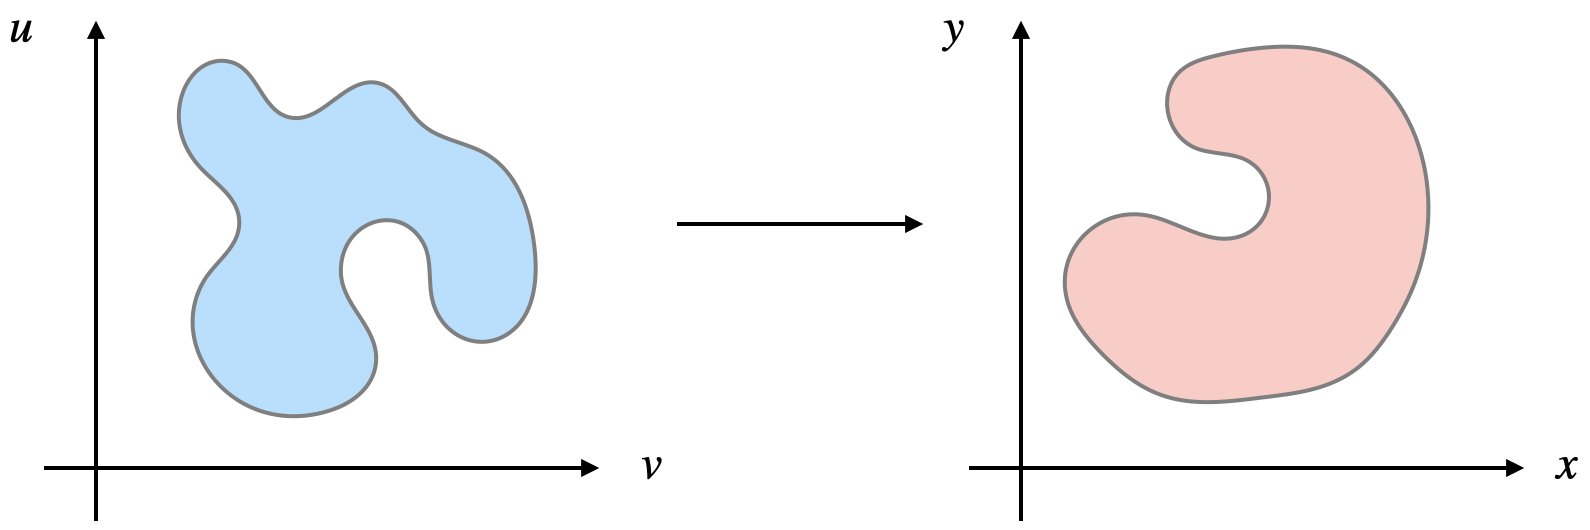
\includegraphics[width=90mm]{var_change0.png}
 \end{center}
\end{figure}
\vspace{-2mm}


\end{frame}


%%%%%%%%%%%%%%%%%%%%%%%%%%%%%%%%%%%%%%%%%%%%%%%%%%%%%%%%%%%%%%%%%%%%%%%%%%%%%%%%%%%%%%%
%%%%%%%%%%%%%%%%%%%%%%%%%%%%%%%%%%%%%%%%%%%%%%%%%%%%%%%%%%%%%%%%%%%%%%%%%%%%%%%%%%%%%%%


\begin{frame}
\frametitle{ヤコビアン}

変数変換$x=\phi(u,v), y=\psi(u,v)$のヤコビアンを
$$
J
=\frac{\partial(x,y)}{\partial(u,v)}=\frac{\partial x}{\partial u}\frac{\partial y}{\partial v}-\frac{\partial x}{\partial v}\frac{\partial y}{\partial u}
$$
で定義する. 
ヤコビアンは$u,v$の関数であり, $J(u,v)$や$\frac{\partial(x,y)}{\partial(u,v)}$とも書かれる. 
ヤコビアンの正体はヤコビ行列
$\begin{bmatrix}\frac{\partial x}{\partial u} & \frac{\partial x}{\partial v} \\ \frac{\partial y}{\partial u} &\frac{\partial y}{\partial v} \end{bmatrix}$
の行列式であり, 変数変換における符号付き面積拡大率を表している. 

\end{frame}


%%%%%%%%%%%%%%%%%%%%%%%%%%%%%%%%%%%%%%%%%%%%%%%%%%%%%%%%%%%%%%%%%%%%%%%%%%%%%%%%%%%%%%%
%%%%%%%%%%%%%%%%%%%%%%%%%%%%%%%%%%%%%%%%%%%%%%%%%%%%%%%%%%%%%%%%%%%%%%%%%%%%%%%%%%%%%%%


\begin{frame}
\frametitle{変数変換の公式}


\begin{Thm} \label{二重積分_変換公式}
$uv$平面内の領域$E$と$xy$平面内の領域$D$の間の変数変換$x=\phi(u,v)$, $y=\psi(u,v)$に関して, $E$上で$J\ne0$であるとき
$$
\iint_D f(x,y)dxdy = \iint_E f(\phi(u,v),\psi(u,v))|J|dudv. 
$$
($|J|$は$J$の絶対値.) 
\end{Thm}
$dxdy=|J|dudv$なる置換は, 微小面積の拡大率を表している. 
一変数の場合と異なり, 重積分には積分領域の向きの概念がなくなっており, 符号は高さに押し付けられている. 
そのためヤコビアンに絶対値が付いている.  

\end{frame}



%%%%%%%%%%%%%%%%%%%%%%%%%%%%%%%%%%%%%%%%%%%%%%%%%%%%%%%%%%%%%%%%%%%%%%%%%%%%%%%%%%%%%%%
%%%%%%%%%%%%%%%%%%%%%%%%%%%%%%%%%%%%%%%%%%%%%%%%%%%%%%%%%%%%%%%%%%%%%%%%%%%%%%%%%%%%%%%



\begin{frame}
\frametitle{変数変換の公式}

 
実際には, (1)変数変換の単射性, (2)$J\ne 0$, が成立しない集合が$E$の中で面積$0$であれば, 定理\ref{二重積分_変換公式}は成立する. 

\begin{figure}[htbp]
 \begin{center} 
  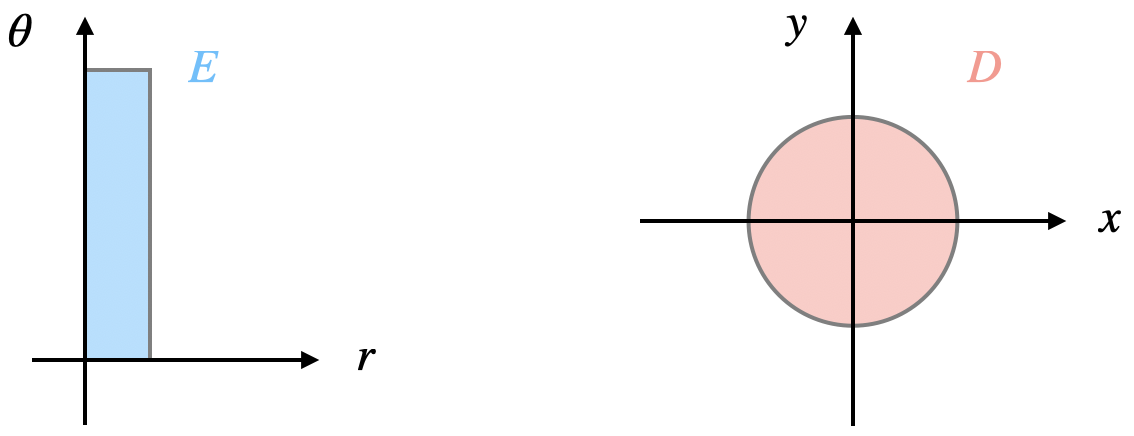
\includegraphics[width=70mm]{polar_coord.png}
 \end{center}
\end{figure}
\vspace{-2mm}

例えば, $E=[0,1]\times [0,2\pi]$と単位円$D$の間の極座標変換
$$
x=r\cos \theta, \ \ \ y=r \sin \theta
$$
に関して
$$
J= \cos \theta \cdot r \cos \theta-(-r\sin \theta)\cdot \sin \theta = r. 
$$
(極座標変換は$E$の境界の一部で単射でなく, また$r=0$で$J=0$である.)

\end{frame}


%%%%%%%%%%%%%%%%%%%%%%%%%%%%%%%%%%%%%%%%%%%%%%%%%%%%%%%%%%%%%%%%%%%%%%%%%%%%%%%%%%%%%%%
%%%%%%%%%%%%%%%%%%%%%%%%%%%%%%%%%%%%%%%%%%%%%%%%%%%%%%%%%%%%%%%%%%%%%%%%%%%%%%%%%%%%%%%



\begin{frame}
\frametitle{変数変換の公式}

領域$D=\{(x,y) \ | \ 0 \le x+y \le 1, 0 \le x-y \le 1\}$上の積分
$$
\iint_D (2x+3y)dxdy
$$
を計算する. $u=x+y$, $v=x-y$, つまり
$$
x=\frac{1}{2}(u+v), \ \ \ y=\frac{1}{2}(u-v)
$$
なる変数変換をすると, $D$は$E=[0,1] \times [0,1]$に対応する. 
\vspace{-2mm}
\begin{figure}[htbp]
 \begin{center} 
  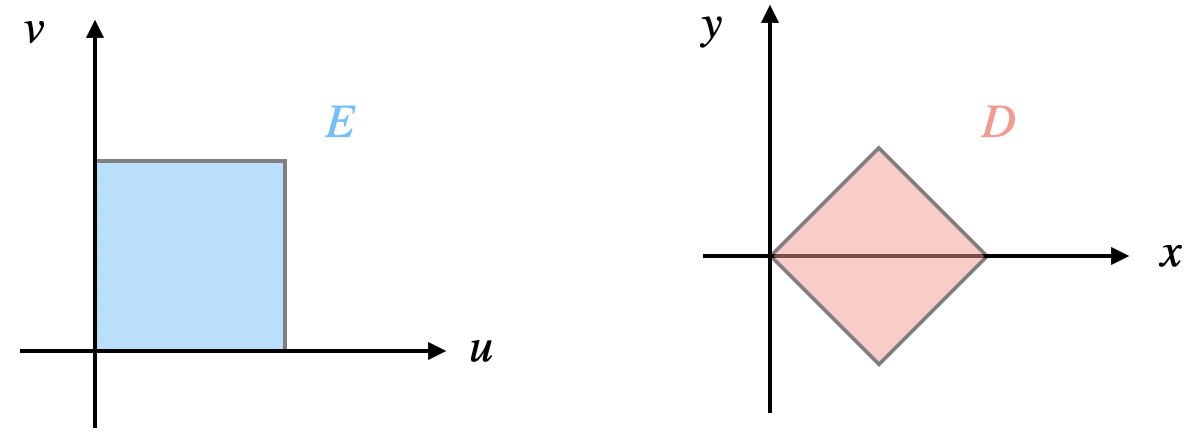
\includegraphics[width=70mm]{var_change.png}
 \end{center}
\end{figure}
\vspace{-2mm}

\end{frame}


%%%%%%%%%%%%%%%%%%%%%%%%%%%%%%%%%%%%%%%%%%%%%%%%%%%%%%%%%%%%%%%%%%%%%%%%%%%%%%%%%%%%%%%
%%%%%%%%%%%%%%%%%%%%%%%%%%%%%%%%%%%%%%%%%%%%%%%%%%%%%%%%%%%%%%%%%%%%%%%%%%%%%%%%%%%%%%%



\begin{frame}
\frametitle{変数変換の公式}

変数変換$x=\frac{1}{2}(u+v), y=\frac{1}{2}(u-v)$に関して, ヤコビアンは
\begin{align*}
J & = \frac{1}{2}\cdot (-\frac{1}{2})-\frac{1}{2} \cdot \frac{1}{2}=-\frac{1}{2}. 
\end{align*}
被積分関数は
\begin{align*}
2x+3y = 2 \cdot \frac{1}{2}(u+v)+3 \cdot \frac{1}{2}(x-y) = \frac{1}{2}(5u-v)
\end{align*}
であるから
\begin{align*}
\iint_D (2x+3y)dxdy & = \iint_E  \frac{1}{2}(5u-v) \frac{1}{2}dudv \\
& = \frac{1}{4} \int_0^1\big( \int_0^1 (5u-v)dv\big)du=\frac{1}{2}.  
\end{align*}
\end{frame}



%%%%%%%%%%%%%%%%%%%%%%%%%%%%%%%%%%%%%%%%%%%%%%%%%%%%%%%%%%%%%%%%%%%%%%%%%%%%%%%%%%%%%%%
%%%%%%%%%%%%%%%%%%%%%%%%%%%%%%%%%%%%%%%%%%%%%%%%%%%%%%%%%%%%%%%%%%%%%%%%%%%%%%%%%%%%%%%



\begin{frame}
\frametitle{変数変換の公式}

領域$D=\{(x,y) \ | \ x^2+y^2 \le 4, y \ge 0\}$上の積分
$$
\iint_D x^2y dxdy
$$
を計算する. 
極座標変換
$$
x=r\cos \theta, \ \ \ y=r \sin \theta
$$
によって
$D$は$E=[0,2] \times [0,\pi]$に対応する. 
またヤコビアンは$J=r$である. 


\begin{figure}[htbp]
 \begin{center} 
  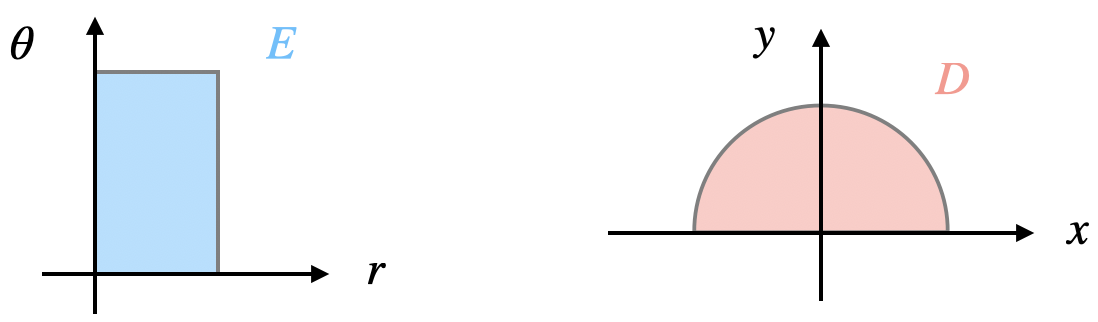
\includegraphics[width=80mm]{polar_coord2.png}
 \end{center}
\end{figure}

\end{frame}


%%%%%%%%%%%%%%%%%%%%%%%%%%%%%%%%%%%%%%%%%%%%%%%%%%%%%%%%%%%%%%%%%%%%%%%%%%%%%%%%%%%%%%%
%%%%%%%%%%%%%%%%%%%%%%%%%%%%%%%%%%%%%%%%%%%%%%%%%%%%%%%%%%%%%%%%%%%%%%%%%%%%%%%%%%%%%%%



\begin{frame}
\frametitle{変数変換の公式}
\begin{align*}
\iint_D x^2y dxdy & = \iint_E (r \cos \theta)^2 r \sin \theta r dr d\theta \\
& = \int_0^\pi \big( \int_0^2 r^4 \cos^2 \theta \sin \theta dr \big) d\theta \\
& = \int_0^\pi \big[ \frac{1}{5}r^5 \cos^2 \theta \sin \theta \big]_{r=0}^2 d\theta \\
& = \int_0^\pi \frac{32}{5} \cos^2 \theta \sin \theta d\theta \\
& = \big[-\frac{32}{15} \cos^3 \theta\big]_0^\pi = \frac{64}{15}. 
\end{align*}

\end{frame}
%%%%%%%%%%%%%%%%%%%%%%%%%%%%%%%%%%%%%%%%%%%%%%%%%%%%%%%%%%%%%%%%%%%%%%%%%%%%%%%%%%%%%%%
%%%%%%%%%%%%%%%%%%%%%%%%%%%%%%%%%%%%%%%%%%%%%%%%%%%%%%%%%%%%%%%%%%%%%%%%%%%%%%%%%%%%%%%

%%%%%%%%%%%%%%%%%%%%%%%%%%%%%%%%%%%%%%%%%%%%%%%%%%%%%%%%%%%%%%%%%%%%%%%%%%%%%%%%%%%%%%%
%%%%%%%%%%%%%%%%%%%%%%%%%%%%%%%%%%%%%%%%%%%%%%%%%%%%%%%%%%%%%%%%%%%%%%%%%%%%%%%%%%%%%%%



\begin{frame}
\frametitle{変数変換の公式}


\begin{Prob}
次の二重積分を計算せよ. 
\begin{enumerate}
\item $D_1=\{(x,y) \ | \ 0 \le -x+2y \le 3, 0 \le 2x-y \le 3\}$
$$\iint_{D_1} (x+y) dxdy$$
\item $D_2=\{(x,y) \ | \  1 \le x^2+y^2 \le 4\}$
$$
\iint_{D_2} \frac{1}{x^2+y^2}dxdy
$$
\end{enumerate}
\end{Prob}

\end{frame}



%%%%%%%%%%%%%%%%%%%%%%%%%%%%%%%%%%%%%%%%%%%%%%%%%%%%%%%%%%%%%%%%%%%%%%%%%%%%%%%%%%%%%%%
%%%%%%%%%%%%%%%%%%%%%%%%%%%%%%%%%%%%%%%%%%%%%%%%%%%%%%%%%%%%%%%%%%%%%%%%%%%%%%%%%%%%%%%



\begin{frame}
\frametitle{変数変換の公式}
変数変換$u=-x+2y$, $v=2x-y$, つまり
$$
x=\frac{1}{3}(u+2v), \ \ \ y=\frac{1}{3}(2u+v)
$$
によって, $E= \{(u,v) \ | \ 0 \le u \le 3, \ 0 \le v \le 3\}$は$D_1$に写される. 
また
$$
J  = \frac{1}{3}\cdot \frac{1}{3}-\frac{2}{3} \cdot \frac{2}{3}=-\frac{1}{3}. 
$$
\begin{figure}[htbp]
 \begin{center} 
  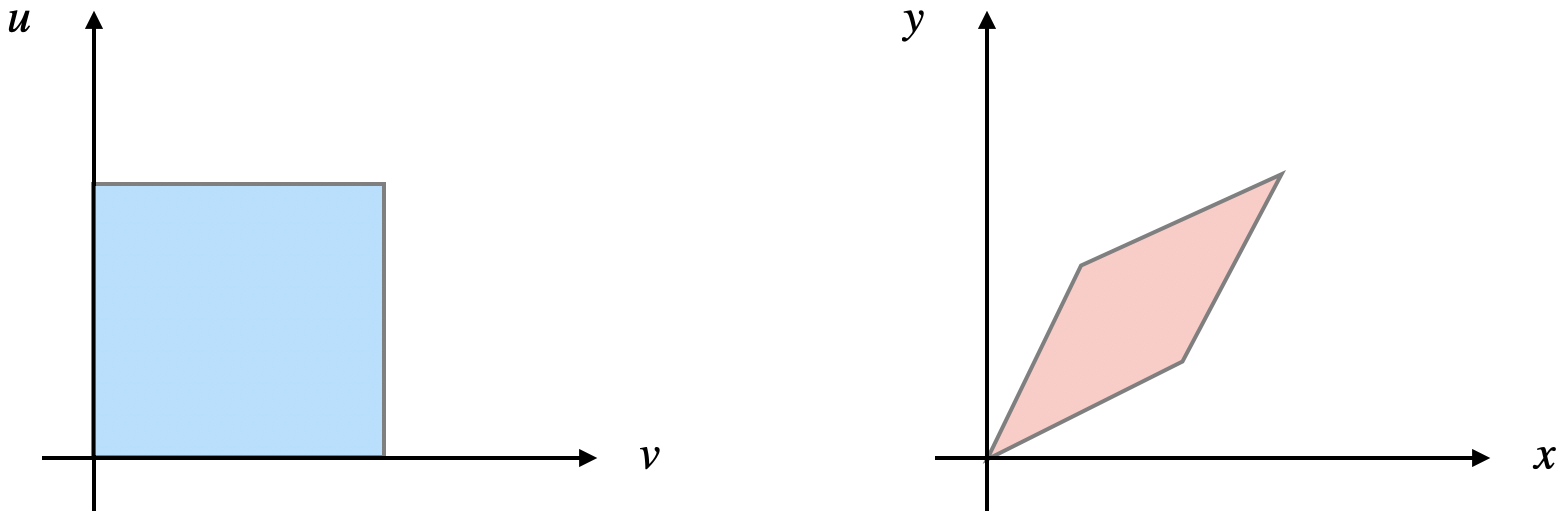
\includegraphics[width=80mm]{skew.png}
 \end{center}
\end{figure}

\end{frame}


%%%%%%%%%%%%%%%%%%%%%%%%%%%%%%%%%%%%%%%%%%%%%%%%%%%%%%%%%%%%%%%%%%%%%%%%%%%%%%%%%%%%%%%%
%%%%%%%%%%%%%%%%%%%%%%%%%%%%%%%%%%%%%%%%%%%%%%%%%%%%%%%%%%%%%%%%%%%%%%%%%%%%%%%%%%%%%%%%

\begin{frame}
\frametitle{変数変換の公式}

したがって
\begin{align*}
\iint_{D_1} (x+y) dxdy & = \iint_E (\frac{1}{3}(u+2v)+\frac{1}{3}(2u+v) ) |-\frac{1}{3}|dudv \\
& = \frac{1}{3} \int_0^3 \int_0^3 (u+v) dudv \\
& = \frac{1}{3}\int_0^3 \big[\frac{1}{2}u^2+uv\big]_{u=0}^3dv  \\
& =  \frac{1}{3}\int_0^3(\frac{9}{2}+3v)dv\\
&= \big[\frac{3}{2}v+\frac{1}{2}v^2\big]_0^3 = 9 
\end{align*}

\end{frame}



%%%%%%%%%%%%%%%%%%%%%%%%%%%%%%%%%%%%%%%%%%%%%%%%%%%%%%%%%%%%%%%%%%%%%%%%%%%%%%%%%%%%%%%%
%%%%%%%%%%%%%%%%%%%%%%%%%%%%%%%%%%%%%%%%%%%%%%%%%%%%%%%%%%%%%%%%%%%%%%%%%%%%%%%%%%%%%%%%
%
%\begin{frame}
%\frametitle{変数変換の公式}
%
%したがって
%\begin{align*}
%\iint_{D_1} 9xy dxdy & = \int_E 9 \cdot \frac{1}{3}(u+2v)\frac{1}{3}(2u+v) \cdot |-\frac{1}{3}|dudv \\
%& = \frac{1}{3} \int_0^3 \int_0^3 (2u^2+5uv+2v^2)dudv \\
%& = \frac{1}{3}\int_0^3 \big[\frac{2}{3}u^3+\frac{5}{2}u^2v+2uv^2 \big]_{u=0}^3dv  \\
%& =  \frac{1}{3}\int_0^3(18+\frac{45}{2}v+6v^2)dv\\
%&= \big[6u+\frac{15}{4}v^2+2v^3\big]_0^3 = \frac{423}{4}. 
%\end{align*}
%
%\end{frame}




%%%%%%%%%%%%%%%%%%%%%%%%%%%%%%%%%%%%%%%%%%%%%%%%%%%%%%%%%%%%%%%%%%%%%%%%%%%%%%%%%%%%%%%
%%%%%%%%%%%%%%%%%%%%%%%%%%%%%%%%%%%%%%%%%%%%%%%%%%%%%%%%%%%%%%%%%%%%%%%%%%%%%%%%%%%%%%%

\begin{frame}
\frametitle{変数変換の公式}

極座標変換$x=r \cos \theta$, $y=r \sin \theta$によって, $E= [1,2] \times [0, 2\pi]$は$D_2$に写される. 
$J=r$であるから

\begin{align*}
\iint_{D_2} \frac{1}{x^2+y^2}dxdy & = \iint_E \frac{1}{(r \cos \theta)^2+(r\sin \theta)^2}r dr d \theta \\
& = \int_0^{2\pi} (\int_1^2 \frac{1}{r}dr) d\theta \\
& = \int_0^{2\pi} \big[ \log|r| \big]_{r=1}^{2}d\theta \\
& = \int_0^{2\pi} \log 2 d\theta \\
& = \big[\theta \log 2\big]_0^{2\pi} = 2\pi \log 2. 
\end{align*}


\end{frame}
%%%%%%%%%%%%%%%%%%%%%%%%%%%%%%%%%%%%%%%%%%%%%%%%%%%%%%%%%%%%%%%%%%%%%%%%%%%%%%%%%%%%%%%
%%%%%%%%%%%%%%%%%%%%%%%%%%%%%%%%%%%%%%%%%%%%%%%%%%%%%%%%%%%%%%%%%%%%%%%%%%%%%%%%%%%%%%%






%%%%%%%%%%%%%%%%%%%%%%%%%%%%%%%%%%%%%%%%%%%%%%%%%%%%%%%%%%%%%%%%%%%%%%%%%%%%%%%%%%%%%%%
%%%%%%%%%%%%%%%%%%%%%%%%%%%%%%%%%%%%%%%%%%%%%%%%%%%%%%%%%%%%%%%%%%%%%%%%%%%%%%%%%%%%%%%

\section{今日のまとめ}
\begin{frame}
\frametitle{まとめ}   


\begin{enumerate}
\item 有界閉領域, 二重積分, 累次積分
\item 変数変換, ヤコビアン
\end{enumerate} 

\end{frame}


\end{document}